
\begin{center}
    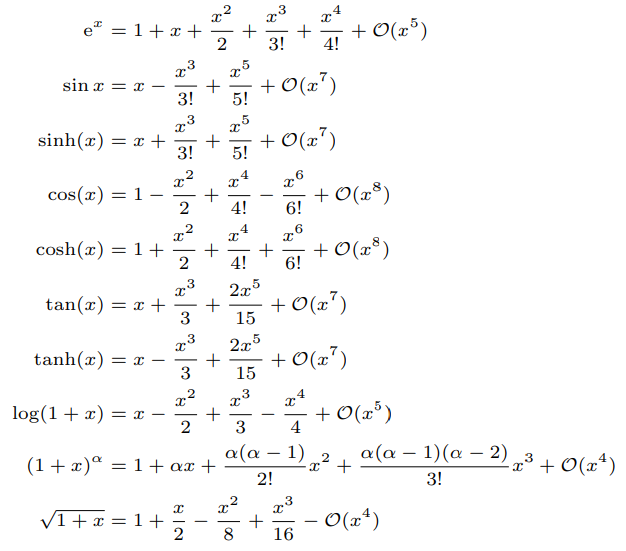
\includegraphics[width=0.8\linewidth]{images/taylorreihen.png}
    \begin{center}

        \subsubsection{Relle Exponentialfunktion}
\begin{center}
    \hfill
    \begin{minipage}{0.3\linewidth}
        \begin{iequation}
            \exp (z) \coloneqq \sum_{n=0}^\infty \frac{z^n}{n!}
        \end{iequation}
    \end{minipage}
    \hfill
    \begin{minipage}{0.6\linewidth}
        \begin{theorem}{Eigenschaften}
            $\exp : \R \to ]0, + \infty[$ ist streng monoton wachsend, stetig und surjektiv.
        \end{theorem}       
    \end{minipage}
    \hfill
\end{center}

%\begin{center}
    \begin{minipage}{0.5\linewidth}
        \begin{iequation}[align*]
            \exp(-x)\exp(x) &= 1\\
	    \text{\textbf{\textsf{}}} \quad\exp(x) &> 0 \qquad\forall x \in \R \tikz[remember picture, overlay]
	    \coordinate(expineq) at (0,0);\\
            \exp(x) &> 1 \qquad\forall x > 0\\
            \exp(a+b) &= \exp(a) \cdot \exp(b)\\ 
            \exp(a-b) &= \exp(a) \div \exp(b)
        \end{iequation}
\begin{tikzpicture}[overlay, remember picture]
	\node[overlaynote, above right = 8mm and 0mm of expineq] (expineqnote) {Aber nicht: $\exp(z) > 0 \quad \forall z \in \C$};
\end{tikzpicture}
    \end{minipage}
    \hfill
    \begin{minipage}{0.48\linewidth}
        \begin{corollary}
            \\$\exp(z) > \exp(y) \quad \forall z > y$
        \end{corollary}
        \begin{corollary}
            \\${\exp (x) \geq 1 + x \quad \forall x \in \R}$
        \end{corollary}    
        \begin{corollary}
            \\$e^{\alpha x} = \sum_{n=0}^\infty \frac{\alpha^n x^n}{n!}$
        \end{corollary}
    \end{minipage}
%\end{center}
$\exp(z) = \exp(y + (z-y)) = \exp(y) \exp(z-y)\\
            \exp(x) = \lim_{n\to \infty}(1 + \frac{x}{n})^n$\\
 \begin{minipage}{0.6\linewidth}
        \begin{align*}
            \exp(\ln a + \ln b) &= \exp(\ln a) \cdot \exp (\ln b)\\
            \exp(\ln a)\exp(\ln b) &= ab = \exp(\ln ab)\\
            \exp(\ln a + \ln b) &= \exp(\ln ab)\\
            \ln a + \ln b &= \ln (ab)
        \end{align*}
    \end{minipage}
    \hfill
    \begin{minipage}{0.35\linewidth}
        \begin{iequation}
            x^a \coloneqq \exp(a \ln x)
        \end{iequation}
    \end{minipage}


    \begin{tabular}{c||c}
        $f(x)$ & $f'(x)$ \\
        \hline$c$ & 0 \\
        $x^{a}$ & $a \cdot x^{a-1}$ \\
        $a^{c x}$ & $a^{c x} \cdot c \ln a$ \\
        $x^{x}$ & $x^{x} \cdot(1+\ln x) \quad x>0$ \\
        $x^{\left(x^{x}\right)}$ & $\left(x^{x}\right)^{x}(x+2 x \ln (x)) \quad x>0$ \\
        $\frac{1}{a+1} x^{a+1}$ & $x^{a}$ \\
        $\frac{1}{f(x)}$ & $\frac{-f^{\prime}(x)}{(f(x))^{2}}$ \\
        $\frac{1}{a \cdot(n+1)}(a x+b)^{n+1}$ & $(a x+b)^{n}$ \\
        $\frac{x^{\alpha+1}}{\alpha+1}$ & $x^{\alpha}, \alpha \neq-1$ \\
        $\sqrt{x}$ & $\frac{1}{2 \sqrt{x}}$ \\
        $\sqrt[n]{x}$ & $\frac{1}{n} x^{\frac{1}{n}-1}$ \\
        $\frac{2}{3} x^{\frac{3}{2}}$ & $\sqrt{x}$ \\
        $\frac{n}{n+1} x^{\frac{1}{n}+1}$ & $\sqrt[n]{x}$ \\
        $e^{x}$ & $e^{x}$ \\
        $\ln (|x|)$ & $\frac{1}{x}$ \\
        $\log { }_{a}|x|$ & $\frac{1}{x \ln a}=\log (e) \frac{1}{x}$ \\
        $\sin (x)$ & $\cos (x)$ \\
        $\cos (x)$ & $-\sin ^{2}(x)$ \\
        $\tan (x)$ & $\frac{1}{\cos ^{2}(x)}=1+\tan ^{2}(x)$ \\
        $\cot (x)$ & $\frac{1}{-\sin ^{2}(x)}$ \\
        $\arcsin (x)$ & $\frac{1}{\sqrt{1-x^{2}}}$ \\
        $\arccos (x)$ & $\frac{-1}{\sqrt{1-x^{2}}}$ \\
        $\arctan (x)$ & $\frac{1}{1+x^{2}}$ \\
          $\ln \left(x+\sqrt{x^{2} \pm a^{2}}\right)$ & $\frac{1}{\sqrt{x^{2} \pm a^{2}}}$ \\
         $\frac{1}{2}(x-\sin (x) \cos (x))$ & $\sin ^{2}(x)$ \\
         $\frac{1}{2}(x+\sin (x) \cos (x))$ & $\cos ^{2}(x)$ \\
          $\tan (x)-x$ & $\tan ^{2}(x)$ \\
         $-\cot (x)-x$ & $\cot ^{2}(x)$ \\
         $x \arcsin (x)+\sqrt{1-x^{2}}$ & $\arcsin (x)$ \\
         $x \arccos (x)-\sqrt{1-x^{2}}$ & $\arccos (x)$ \\
         $x \arctan (x)-\frac{1}{2} \ln \left(1+x^{2}\right)$ & $\arctan (x)$ \\
          $\ln (\cosh (x))$ & $\tanh (x)$ \\
          $\ln |f(x)|$ & $\frac{f^{\prime}(x)}{f(x)}$ \\
         $x \cdot(\ln |x|-1)$ & $\ln |x|$ \\
         $\frac{1}{n+1}(\ln x)^{n+1} \quad n \neq-1$ & $\frac{1}{x}(\ln x)^{n}$ \\
         $\frac{1}{2 n}\left(\ln x^{n}\right)^{2} \quad n \neq 0$ & $\frac{1}{x} \ln x^{n}$ \\
          $\ln |\ln x| \quad x>0, x \neq 1$ & $\frac{1}{x \ln x}$ \\
         $\frac{1}{b \ln a} a^{b x}$ & $a^{b x}$ \\
         $\frac{c x-1}{c^{2}} \cdot e^{c x}$ & $x \cdot e^{c x}$ \\
         $\frac{x^{n+1}}{n+1}\left(\ln x-\frac{1}{n+1}\right) \quad n \neq-1$ & $x^{n} \ln x$ \\
        $\frac{\sin ^{2}(x)}{2}$ &
        $\sin (x) \cos (x)$ \\
        \hline
        \end{tabular}
    
        \begin{highlight}{Wichtige Stammfunktionen}
            $\int f(x) \Longrightarrow F(x) + C$
        \begin{center}
            \begin{minipage}{0.45\linewidth}
                \tcbsubtitle{Potenzfunktionen}
                \begin{align*}
                    &\int x^n \dif x  &=&  \quad \frac{1}{n+1}x^{n+1}  \\
                    &\int \frac{f'}{f} \dif x  &=&  \quad \ln \left\lvert f \right\rvert  \\
                    &\int \frac{1}{x} \dif x  &=& \quad \ln \left\lvert x \right\rvert  \\
                    &\int \frac{1}{x+a} \dif x  &=&  \quad \ln \left\lvert x+a \right\rvert \\
                    &\int \frac{1}{(x+a)^2} \dif x  &=&  -\frac{1}{x+a}  \\
                    &\int \frac{1}{\sqrt{x}}\dif x  &=&  2 \sqrt{x}  \\
                \end{align*}
            \end{minipage}
            \hfill\vline\hfill
            \begin{minipage}{0.45\linewidth}
                \tcbsubtitle{Exponential- und Logarithmusfunktionen}
                \begin{align*}
                    &\int\left(e^{x}\right) d x  &=& e^{x} \\
                    &\int e^{ax} \dif x  &=&  \frac{1}{a} e^{ax}  \\
                    &\int\left(a^{x}\right) d x \quad  &=& \frac{a^{x}}{\ln (\mathrm{a})} \\
                    &\int(\ln (x)) d x  &=& x \cdot \ln (x)-x \\
                    &\int\left(\log _{a}(x)\right) d x  &=& \frac{x \cdot \ln (x)-x}{\ln (\mathrm{a})} \\
                \end{align*}
            \end{minipage}
        \end{center}
        \tcbsubtitle{Geometrische Funktionen}
        \begin{center}
            \begin{minipage}{0.4\linewidth}
                    \begin{align*}
                        &\int\cos (x) d x  &=& \sin (x) \\
                        &\int\sin (x) d x  &=& -\cos (x) \\
                        &\int\tan (x) d x  &=& -\ln |\cos (x)| \\
                        &\int \sin(ax)\dif x  &=&  - \frac{1}{a} \cos(a x)  \\
                        &\int \sin^2(ax)\dif x  &=&  \frac{x}{2} - \frac{1}{4a} \sin(2 a x)  \\
                        &\int \cos(ax)\dif x  &=&  \frac{1}{a} \sin(a x)  \\
                        &\int \cos^2(ax)\dif x  &=&  \frac{x}{2} + \frac{1}{4a} \sin(2 a x)  \\
                    \end{align*}
            \end{minipage}
            \hfill\vline\hfill
            \begin{minipage}{0.45\linewidth}
                \begin{align*}
                        &\int\frac{1}{1+\mathrm{x}^{2}} d x  &=& \arctan (\mathrm{x})\\
                        &\int\frac{1}{\sqrt{1-x^{2}}} d x  &=& \arcsin (x) \\
                        &\int -\frac{1}{\sqrt{1-x^{2}}} d x  &=& \arccos (x) \\
                        &\int \frac{1}{\sqrt{1-x^2}}\dif x  &=&  \arcsin(x)  \\
                        &\int -\frac{1}{\sqrt{1-x^2}}\dif x  &=&  \arccos(x)  \\
                        &\int \frac{1}{1+x^2}\dif x  &=&  \arctan(x)  \\
                \end{align*}
            \end{minipage}
        \end{center}
    \end{highlight}